\iffalse
%%%%%%%%%%
%%%% ALT DERZEIT NICHT IM PDF

Klimawandel, Ressourcenverknappung und zunehmende Umweltveränderungen lassen die Transformation des Energiesystems zu einer der zentralen gesellschaftlichen Herausforderungen werden. Noch ist weitgehend offen, wie die Versorgung mit Strom, Wärme, Mobilität sichergestellt werden kann, während Klimaziele erreicht, soziale Gerechtigkeit gewahrt und die natürlichen Grenzen unseres Planeten langfristig eingehalten werden können. 

Energiesystem-Modelle haben sich als Werkzeuge etabliert, um technisch mögliche und ökonomisch vorteilhafte Energiewende-Pfade darzustellen und zu analysieren. Sie helfen dabei, komplexe Zusammenhänge zwischen technischen Möglichkeiten (z.B. Flexibilität), Umweltbedingungen (z.B. Wetter-abhängige Erneuerbare), Marktregeln (z.B. Energy-only-Markt) im Licht klimapolitischer Zielsetzungen zu verstehen und unterstützen somit die Klima- und Energiepolitik.

Ein entscheidender Einflussparameter für berechnete Szenarien ist die zukünftige Nachfrage nach Strom, Wärme und Mobilität. Die Mehrzahl der bisherigen Modelle legt den Fokus  auf die Bereitstellung von Energiedienstleistungen. Die Nachfrage-Seite wird meist nur innerhalb enger Grenzen variiert. So berücksichtigen viele Modelle beispielsweise die Verschiebung der Nachfrage von fossilen Brennstoffen zu Strom durch die Elektifizierung im Wärme- und Transportsektor. Eine übergreifende Perspektive, welche die verschiedenen Bereiche berücksichtigt und integriert, in denen Energie gebraucht wird, steht noch aus. Zudem wird in den meisten Modellen die absolute Nachfrage nach Energie nicht in Frage gestellt. Mit anderen Worten: Bislang sind Modellierungen weitgehend blind gegenüber Veränderungen der Nachfrage nach Energie durch gesellschaftlichen Wandel oder Verhaltensänderungen.

Nicht nur in der Modellierung von Energiewende-Pfaden, sondern auch  bei Klimaschutz-Strategien liegt der Fokus bisher auf im weitesten Sinn technikorientierten Lösungen bei der Erzeugung und Distribution von Energie für Wohnen, Bauen, Ernährung und Mobilität \cite{Creutzig2018}. 

Zwar bieten laut Modellrechnungen Erneuerbare Energien und Effizienz die Möglichkeit im Jahr 2050 80-95 Prozent Treibhausgas-Reduktion in Deutschland \cite{BMWi2017} zu erreichen. Es gibt jedoch verschiedene Gründe keine der drei Nachhaltigkeitsstrategien Konsistenz (Erneuerbare Energien ersetzen Fossile), Effizienz (relative Reduktion des Energieverbrauchs bei Bereitstellung der gleichen Energiedienstleistung) und Suffizienz (absolute Reduktion der Nachfrage nach Energiedienstleistungen durch veränderte soziale Praktiken und gesellschaftliche Leitbilder) außer Acht zu lassen: Zum einen setzten die ambitionierten Ziele des Pariser Klimaabkommens die Herausforderung nochmal auf eine neue Stufe \cite{Rogelj2018}. Außerdem sprechen Aspekte wie Flächenverbrauch (Referenz fehlt noch), Ressourcenbedarf (\url{http://onlinelibrary.wiley.com/doi/10.1002/cite.201400121/full} und \url{https://www.oeko.de/oekodoc/1334/2011-449-de.pdf}) und Akzeptanzfragen \cite{Fuchs2016}, zusammengefasst die Einhaltung der planetaren Grenzen \cite{Rockstroem2009} dafür, die Chancen, die Suffizienz bietet, nicht zu übersehen \cite{SAMADI2017}.

Desweiteren ist bisher nicht abschließend geklärt, in welchem Ausmaß Emissionsreduktionen in Deutschland durch Konsistenz und Effizienz tatsächlich erreicht wurden. Verlagerungseffekte in andere Länder könnten ebenso eine Rolle gespielt haben \cite{Wiedmann2015}, so dass die Emissionsreduktionen bei Bilanzierung nach Verursacherprinzip geringer ausfallen würden (eine weitere Studie, die auf Verlagerungseffekte von Annex B Staaten des Kyoto Protokols in Bezug auf CO2 abhebt, wäre diese hier: \url{https://www.sciencedirect.com/science/article/pii/S0095069611001422}). Auch die Rolle, die Effizienz spielen kann, ist nicht klar. Zielszenarien für Deutschland gehen von einer Reduzierung der Stromnachfrage durch eine massive Steigerung von Effizienz aus \cite{BMWi2017}. Zugleich findet jedoch in der fachwissenschaftlichen und energiepolitischen Diskussion der Befund Aufmerksamkeit, dass Energieeffizienzsteigerungen in der Regel von Rebound-Effekten begleitet werden, welche die Einsparungen teilweise kompensieren oder mitunter sogar zu einem verstärkten Energieverbrauch („Backfire“) führen \cite{DeutscherBundestag2013,Santarius2012}. Auch aufgrund solcher Rebound-Effekte wurden in den vergangenen Jahren die Energiesparpotenziale nicht voll ausgeschöpft, was dazu beitrug, dass in Deutschland trotz aller Maßnahmen zur Verbesserung der Energieeffizienz der Stromverbrauch im Jahr 2016 gegenüber 2008 (acht Jahre) um nur 1,5 Prozent gesunken ist \cite{UBA2017}. Dies lässt das erklärte Ziel weitere 8,5 Prozent bis 2020 (vier Jahre) zu schaffen sehr ambitioniert erscheinen.

In Anbetracht des möglichen Beitrags der Suffizienz und der Größe der Herausforderung, ist die Rolle von Energie-Suffizienz derzeit unterrepräsentiert in Diskussion und Forschung für Klimaschutz und Energiewende. Abbildung \ref{fig:zusammenspiel} verdeutlicht schematisch den Gedanken des Zusammenspiels der drei Dimensionen für die Erreichung der Klimaziele. 


\begin{figure}[!h]
    \centering
    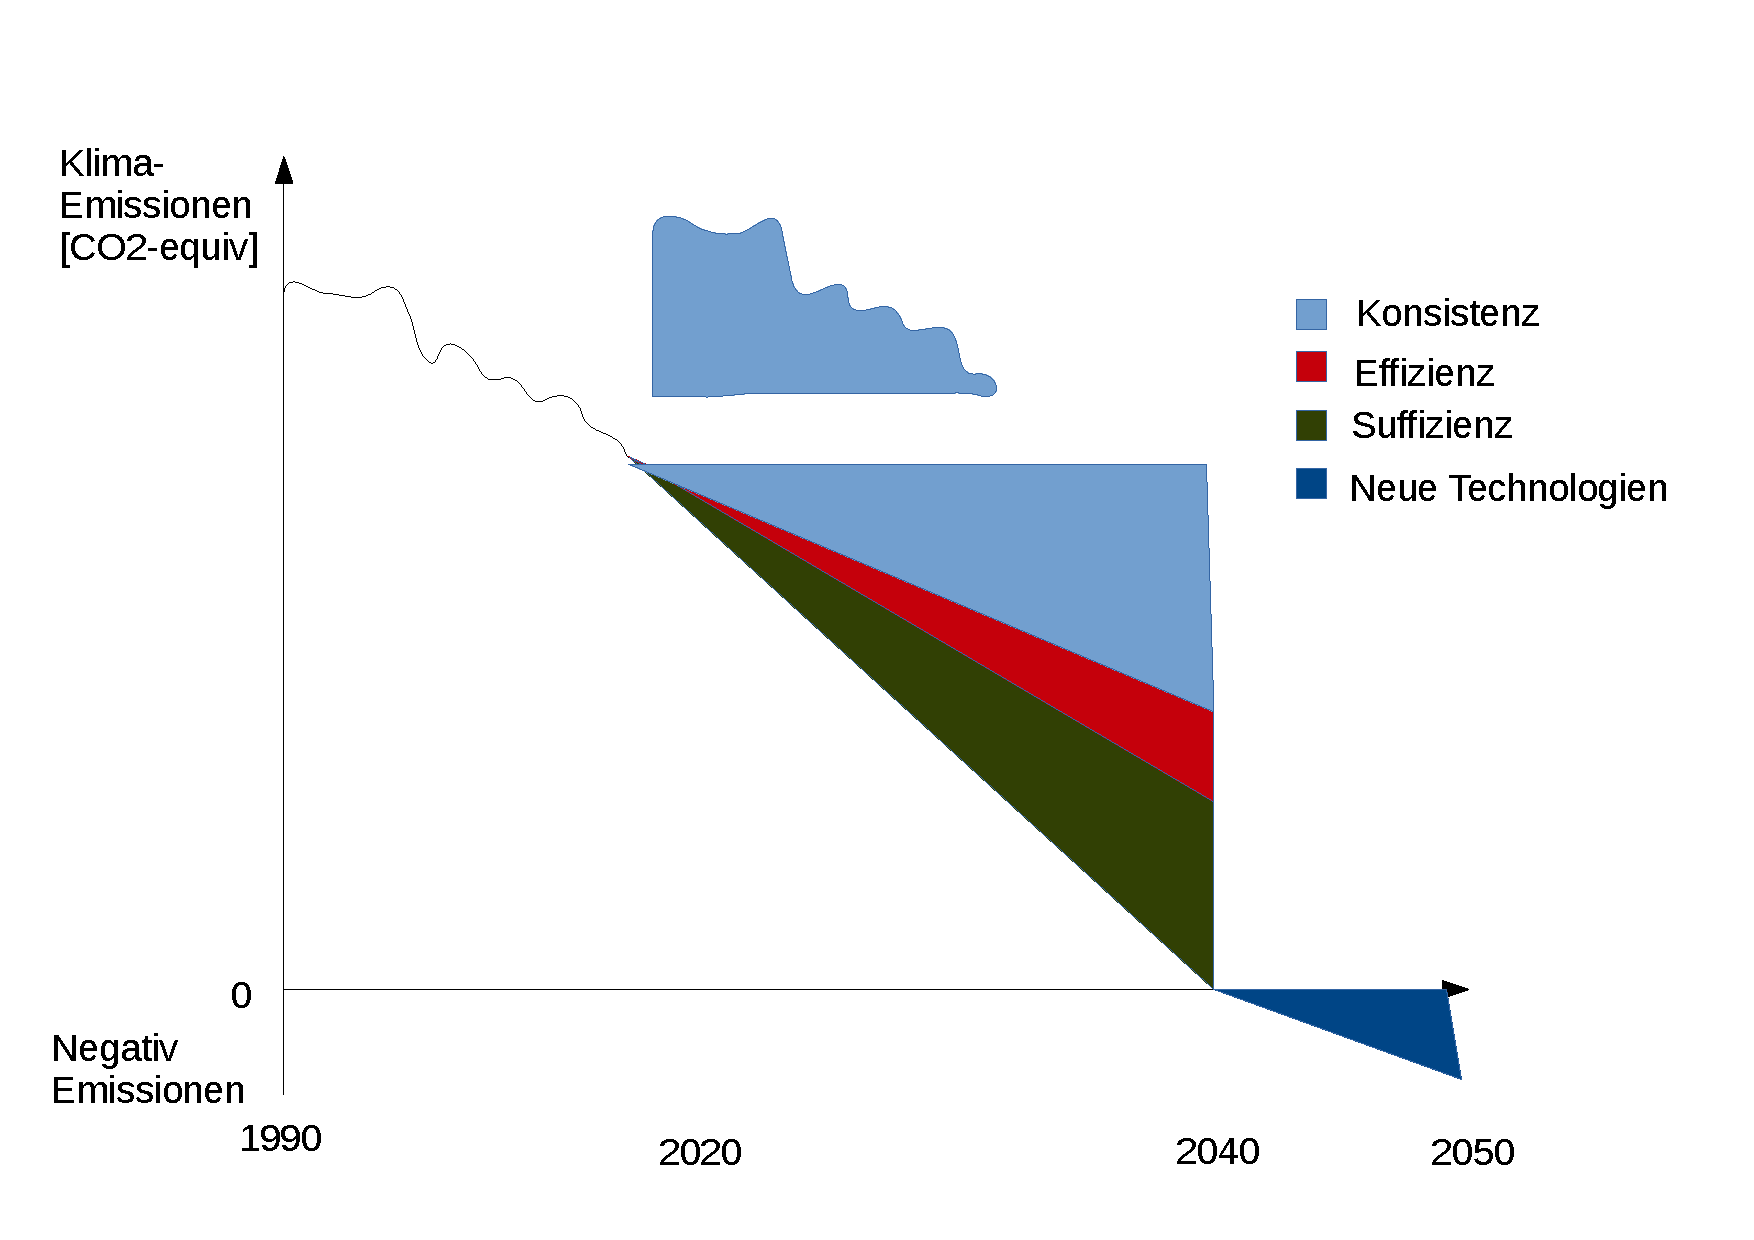
\includegraphics[width=0.8\textwidth]{figures/Zusammenspiel2.pdf}
    \caption{Schamatisch: Bisherige Emissionsreduktion durch Konsistenz (links), notwendiger Beitrag von Effizienz und Suffizienz in Zukunft (rechts) zur Erreichung der Klimaziele in Deutschland}
    \label{fig:zusammenspiel}
\end{figure}

Weiter hat sich in der Forschung die Erkenntnis durchgesetzt, dass sich nur unter Einbeziehung und dem Zusammenspiel verschiedener Disziplinen - wie technisch-/ingenieurwissenschaftlicher Fachrichtungen, Politik-, Wirtschafts- und Sozialwissenschaften - die gesellschaftliche Herausforderung der Transformation des Energiesystems erfolgreich bewältigen lässt \cite{WGBU2011}.

Besonders deutlich wird die Notwendigkeit der verstärkten interdisziplinären Zusammenarbeit bei der Erstellung von Energie-Szenarien. Gesellschaftliche Entwicklungen haben enormen Einfluss auf die Nachfrage nach Energie-Dienstleistungen, die politischen Rahmenbedingungen für die Erzeugungs- und Distributionswege sowie die technisch-ökonomischen Optionen zur Erfüllung der Energienachfrage (schematisch dargestellt in Abbildung \ref{fig:szenarien}). Gängige Praxis in der Energiesystem-Modellierung ist es, nur Letzteres in den Blick zu nehmen, gesellschaftliche Dynamiken hingegen weitgehend zu ignorieren (Abbildung \ref{fig:szenarien} links). Dieses Vorgehen erlaubt eine Abschätzung der Leistungsfähigkeit sozio-technischer Innovationen. Allerdings um den Preis einer Vorstellung, die Gesellschaft als mehr oder weniger statisches Konstrukt imaginiert und nicht als das hoch dynamische, beständigen Veränderungen unterworfene Gemeinwesen, das sie ist. Für konsistente und damit belastbare Energie-Szenarien ist die Integration sozialwissenschaftlicher Wissensbestände in Bezug auf künftig zu erwartende gesellschaftliche Transformationsprozesse und ihre Auswirkungen auf den gesellschaftlichen Metabolismus unverzichtbar. Beispielhaft seien hier die Digitalisierung oder der demografische Wandel genannt. Beide Prozesse werden mit hoher Wahrscheinlichkeit Auswirkungen auf die Nachfrage nach Energiedienstleitungen haben, in welchem Umfang und in welche Richtung - steigende oder sinkende Nachfrage - ist erstens kontingent und zweitens allein mit Verweis auf die Leistungsfähigkeit technischer Innovationen nicht zu beantworten. Noch nicht abzusehen ist auch, in welchem Ausmaß etwa kommunale und nationale Klimaschutzmaßnahmen - erinnert sei hier an die aktuelle Diskussion um den ticketlosen ÖPNV - soziale Innovationen oder einen Wandel gesellschaftlicher Werte und Normen beeinflussen werden. Außerdem ermöglicht die Erweiterung des Bezugsrahmens um die gesellschaftliche Perspektive (Abbildung \ref{fig:szenarien} rechts), Suffizienz neben Effizienz und Konsistenz in der Modellierung abzubilden. 

\begin{figure}[!h]
    \centering
    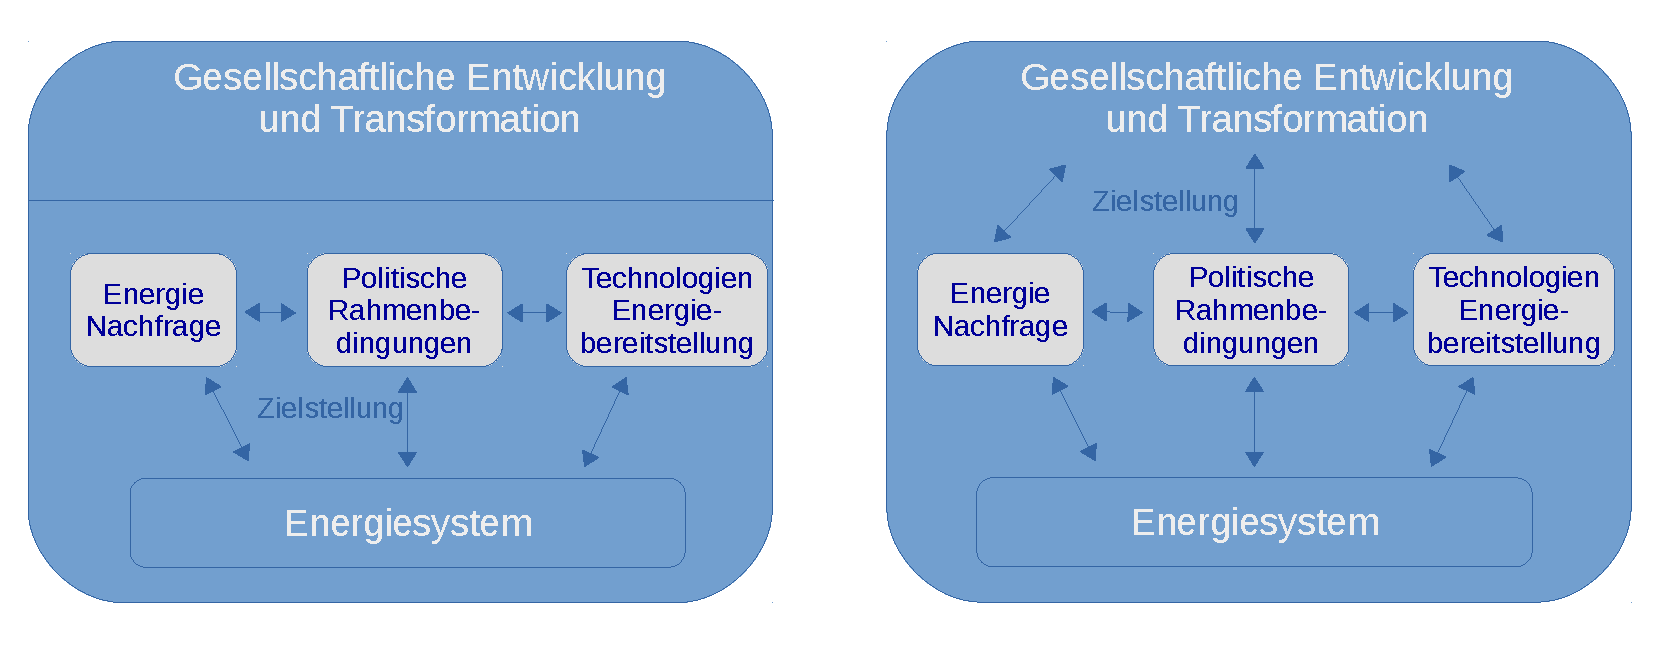
\includegraphics[width=0.8\textwidth]{figures/Szenarien.pdf}
    \caption{Rahmen für Energie-Szenarien: Links: Getrennte Betrachtung / Rechts: Einbettung der Annahmen für Energie-Nachfrage, Politikrahmen und technische Optionen in gesellschaftliche Entwicklungen}
    \label{fig:szenarien}
\end{figure}

Ziele der Nachwuchsforschungs-Gruppe Energie-Suffizienz sind:
\begin{itemize}
 \item Einen in der bisherigen Diskussion um die Transformation des Energiesystems in Richtung Nachhaltigkeit unterrepräsentierten Aspekt  -- Suffizienz -- intensiv dahingehend zu erforschen
  \item In der interdisziplinäre Kooperation ein Verfahren für die Erstellung von konsistenten, multiperspektivischen  Energieszenarien zu entwickeln und zu erproben
  \item (Weiter)-Entwicklung eines Energiesystem-Modells, in dem Konsistenz, Effizienz und Suffizienz integriert betrachtet werden können
 \item Einen möglichen und eventuell notwendigen Beitrag von Energie-Suffizienz zur Erreichung der Klimaziele auf nationaler (Deutschland) und beispielhaft kommunaler Ebene ermitteln
 \item Die Entwicklung von Zukunftsszenarien zur Transformation des Energiesystems in Richtung Nachhaltigkeit 
 \item Die historische Rekonstruktion der Wechselwirkung zwischen Energiesystemtransformation und gesellschaftlichem Wandel  
 \item Handlungsoptionen für Suffizienz-Politik von kommunaler bis EU-Ebene
 \item Literatur und Methoden der Energiesystem-Analyse als auch die der sozial-ökologischen Transformationsforschung erweitern. Schwerpunkt liegt dabei auf Synergien zwischen den Forschungsgebieten.
 \item Das Methodenspektrum junger Forscher mit Hintergründen aus Sozialwissenschaft (sozial-ökologische Transformationsforschung), Wirtschaftingenieurwesen (Energiesystem-Analyse) und Politikwissenschaft interdisziplinär erweitern
\end{itemize}

Im Rahmen des Projektes erarbeitete Daten und Software, werden open source zur Verfügung gestellt. Der Open Science Ansatz, der der Nachwuchs-Forschungsgruppe zugrunde liegen wird, beinhaltet auch den offenen Zugang zu Publikationen etc. Die Erkenntnisse sollen außerdem politische Entscheidungsprozesse zu Klimaschutz und Energiewende unterstützen und Empfehlungen für Suffizienzpolitik beinhalten. Ein Schwerpunkt wird die Ergebnis-Kommunikation auch im populär-wissenschaftlichen Bereich, um auch eine außerwissenschaftliche Öffentlichkeit zu erreichen.
\fi


UTAS VERSION

%In Anlehnung an Albert Einstein liegt der Ausgangspunkt des Nachwuchsforschungsvorhabens darin, dass Probleme nicht mit derselben Rationalität gelöst werden können, die sie hervorgebracht haben. Zwar ist die zentrale Herausforderung einer Energiewende in Deutschland angesichts von Klimawandel, Ressourcenverknappung und Risikotechnologien erkannt, doch die Debatten und Maßnahmen zum Umgang damit verbleiben überwiegend in alten Rationalitätsmustern: Die Energiewende wird unter den Aspekten von Kosten, Marktpotenzialen (einschließlich neuen Geschäftsfeldern) und technischer Machbarkeit (Effizienz und Konsistenz) verhandelt, während „Treiber“ vermehrten Energieverbrauchs, wie das modernen Gesellschaften inhärente Wachstumsparadigma oder zunehmende Innovationsgeschwindigkeit (aufgrund der Verfügbarkeit günstiger Rohstoffe), kaum problematisiert werden. Energiesystem-Modelle haben sich als Werkzeuge etabliert, um technisch mögliche und ökonomisch vorteilhafte Energiewende-Pfade im Zusammenspiel von Effizienz- und Konsistenz-Strategien abzubilden. Entwicklungen, die eine Reduktion des absoluten Energieverbrauchs durch veränderte Praktiken und Routinen im Sinne einer Suffizienz-Strategie ermöglichen, werden bisher in diesen Modellen kaum berücksichtigt \cite{SAMADI2017}. Die Nachfrage-Seite wird in bestehenden Modellen in der Regel über technologische Änderungen (Effizienzmaßnahmen) abgebildet. Die Nachfrage selbst wird üblicherweise nicht hinterfragt \cite{Creutzig2018}, nur innerhalb enger Grenzen variiert und die dahinter liegenden Annahmen werden nicht explizit gemacht. Ein entscheidender Einflussparameter für berechnete Szenarien ist aber die zukünftige Nachfrage nach Strom, Wärme und Mobilität. Mit anderen Worten: Bislang sind Modellierungen weitgehend blind gegenüber Veränderungen durch gesellschaftlichen Wandel und soziale Innovationen und berücksichtigen hier liegende Potenziale und Risiken nicht. Zudem kommen eng mit der Energiewende verknüpfte Aspekte wie Ressourcenbedarf \cite{Mocker2015,Buchert2011} Akzeptanzfragen \cite{Fuchs2016} und Flächenverbrauch , zusammengefasst die Einhaltung der planetaren Grenzen \cite{Rockstroem2009} und eine nachhaltige Entwicklung im Sinne der Sustainable Development Goals \cite{UN_SDG} unberücksichtigt.\\
%Vor diesem Hintergrund liegt das übergreifende Ziel des angestrebten Nachwuchsverbundes darin, Suffizienzaspekte und -strategien für die Energiesystem-Modellierung zu operationalisieren und damit verhaltensbasierte Parameter und gesellschaftlichen Wandel in Energie- und Klimaschutzszenarien abbildbar zu machen. Die Parameter werden dabei mit Instrumenten, Handlungsoptionen und veränderten Rahmenbedingungen explizit hinterlegt. Hierfür gilt es, gesellschaftliche Transformationsprozesse im Kontext der Energiewende besser zu verstehen, die Blockaden für und Potenziale von Suffizienzpolitiken auszuloten und nicht zuletzt im Sinne einer globalen Nachhaltigkeit mögliche Externalisierung und Verlagerungseffekte zu diskutieren.